% --
% spectogram

\section{Spectral Features}\label{sec:signal_spec}
Spectral Features, such as a spectogram, are the most intuitive form to represent audio data. 
They show which frequencies are active at a time instance sampled at the hop time, the time on which the analytic window is shifted forward.

A spectogram with linear representation is shown in \rfig{spec-lin}.

\begin{figure}[!ht]
  \centering
    \subfigure[left]{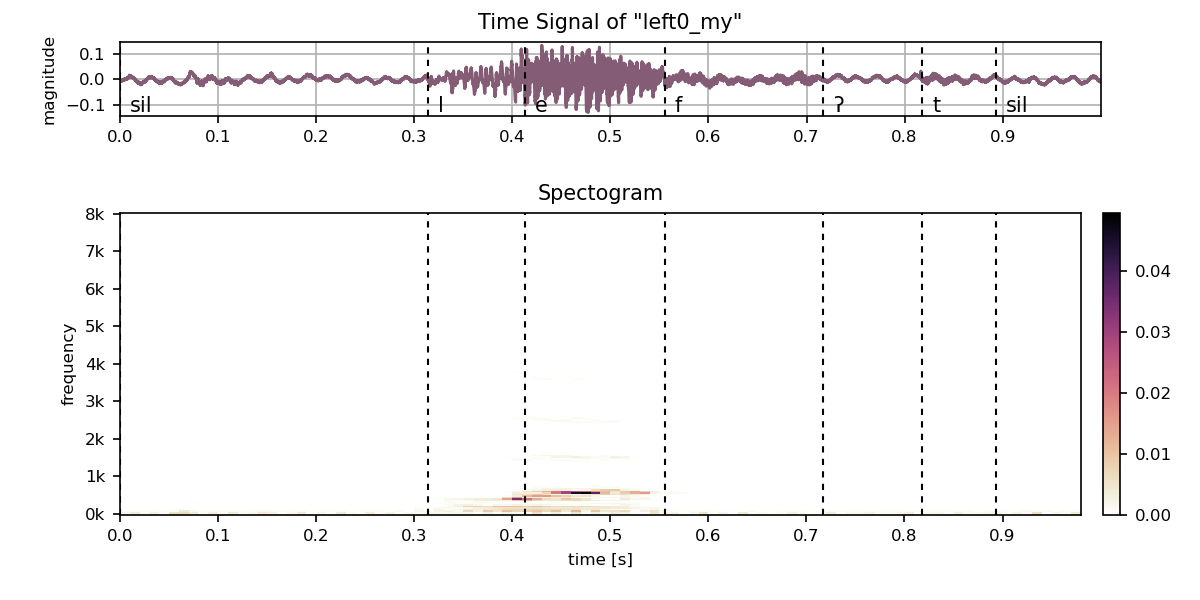
\includegraphics[width=0.45\textwidth]{./3_signal/figs/signal_spec-lin_left0_my}}
    \subfigure[right]{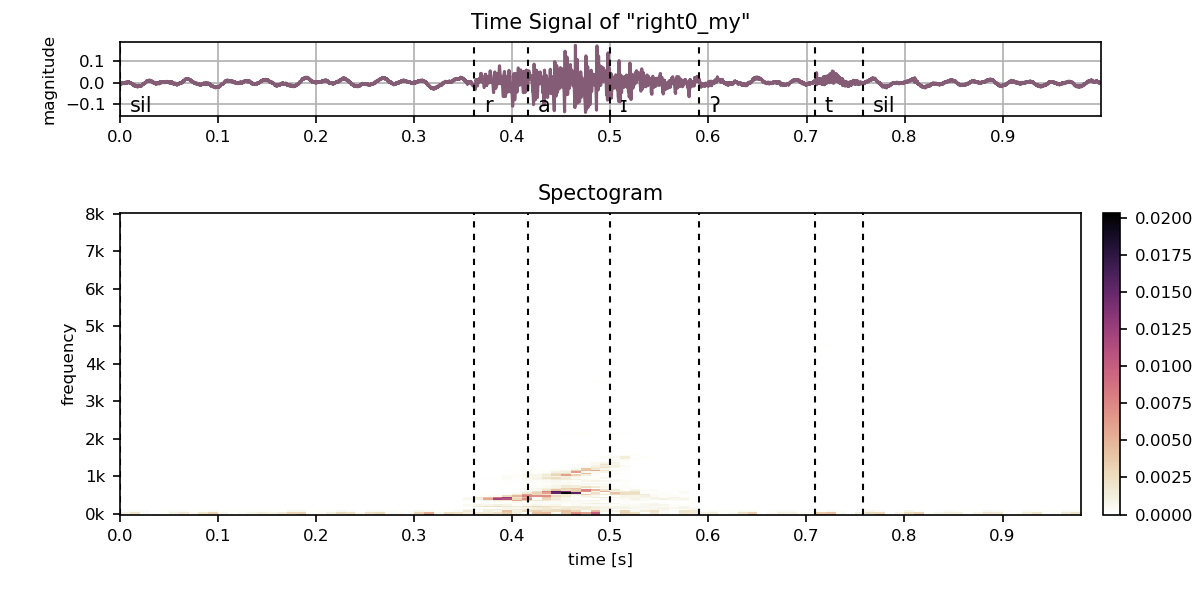
\includegraphics[width=0.45\textwidth]{./3_signal/figs/signal_spec-lin_right0_my}}
    \subfigure[up]{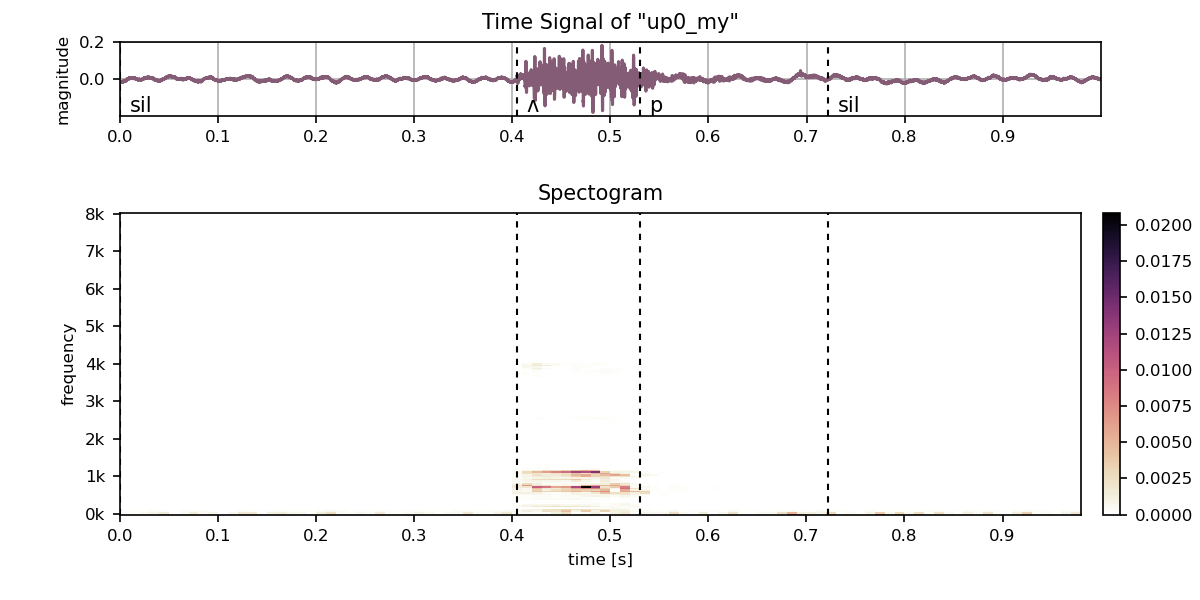
\includegraphics[width=0.45\textwidth]{./3_signal/figs/signal_spec-lin_up0_my}}
    \subfigure[down]{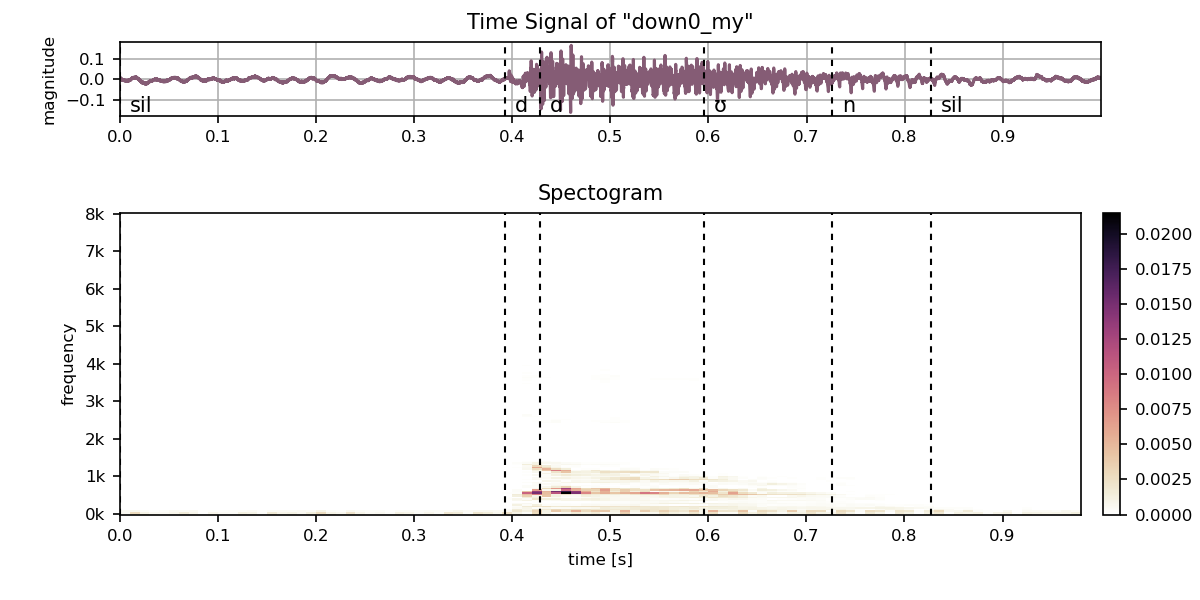
\includegraphics[width=0.45\textwidth]{./3_signal/figs/signal_spec-lin_down0_my}}
    \subfigure[go]{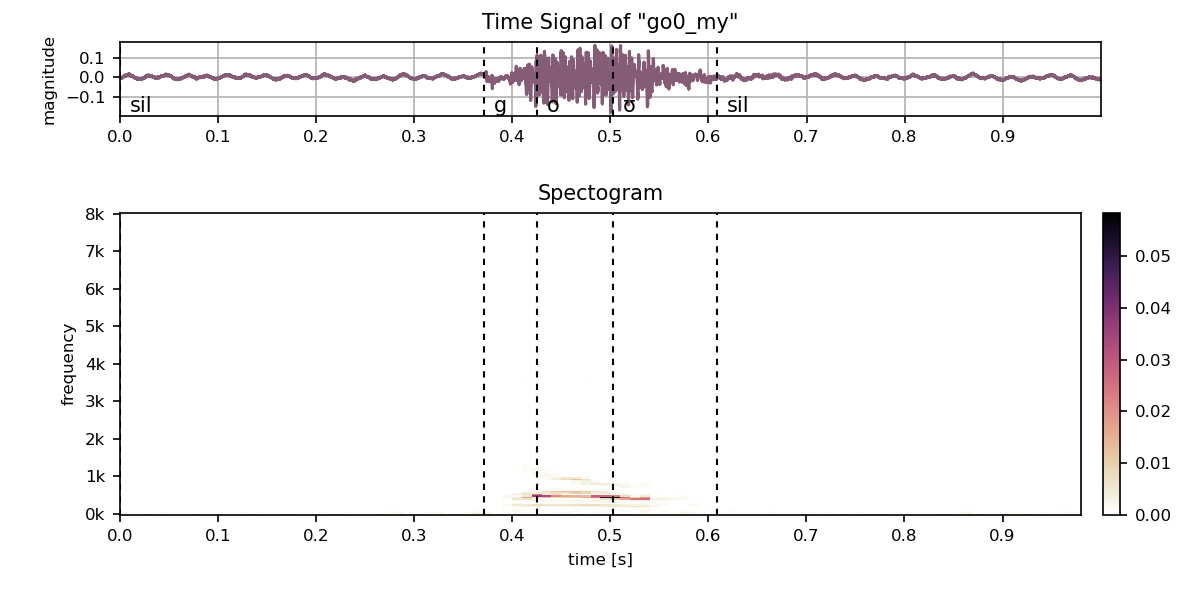
\includegraphics[width=0.45\textwidth]{./3_signal/figs/signal_spec-lin_go0_my}}
  \caption{Spectogram linear scaled.}
  \label{fig:spec-lin}
\end{figure}
\FloatBarrier
\noindent

One can see here, that most of the energy of the signal is in the lower frquency regions under 1kHz.
It is more interesting to go into the log scale, shown in \rfig{spec-log}

\begin{figure}[!ht]
  \centering
    \subfigure[left]{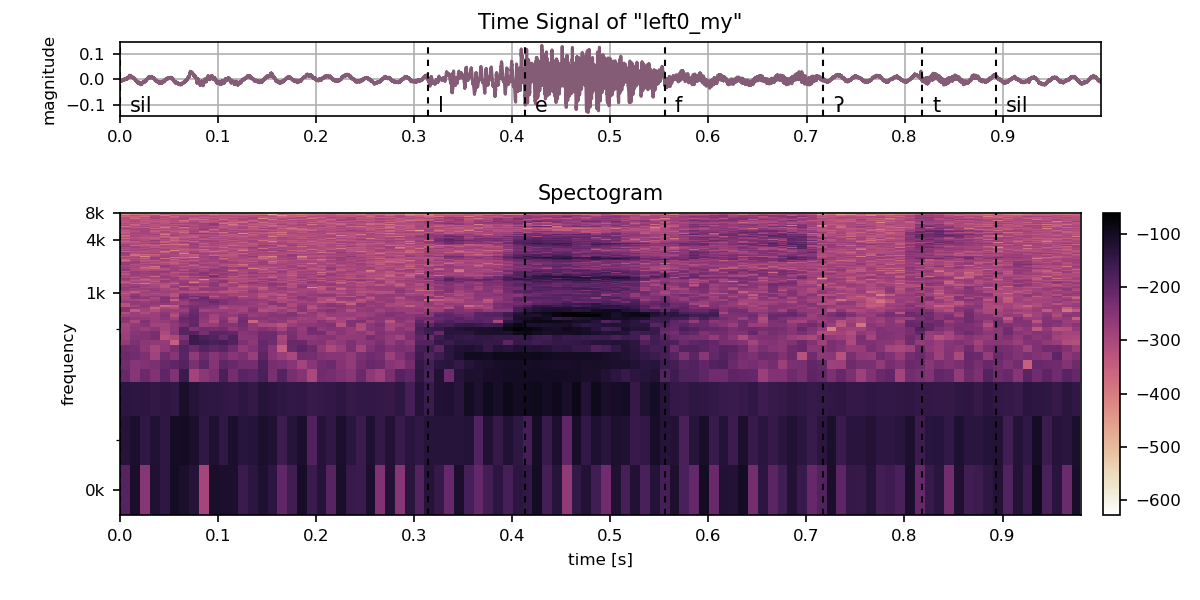
\includegraphics[width=0.45\textwidth]{./3_signal/figs/signal_spec-log_left0_my}}
    \subfigure[right]{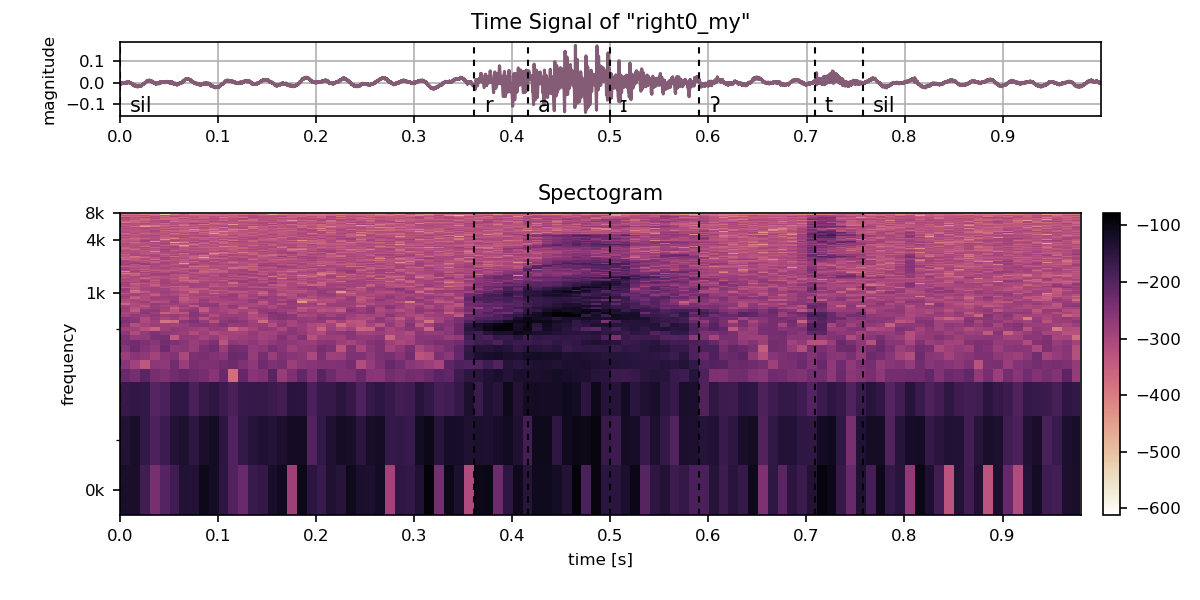
\includegraphics[width=0.45\textwidth]{./3_signal/figs/signal_spec-log_right0_my}}
    \subfigure[up]{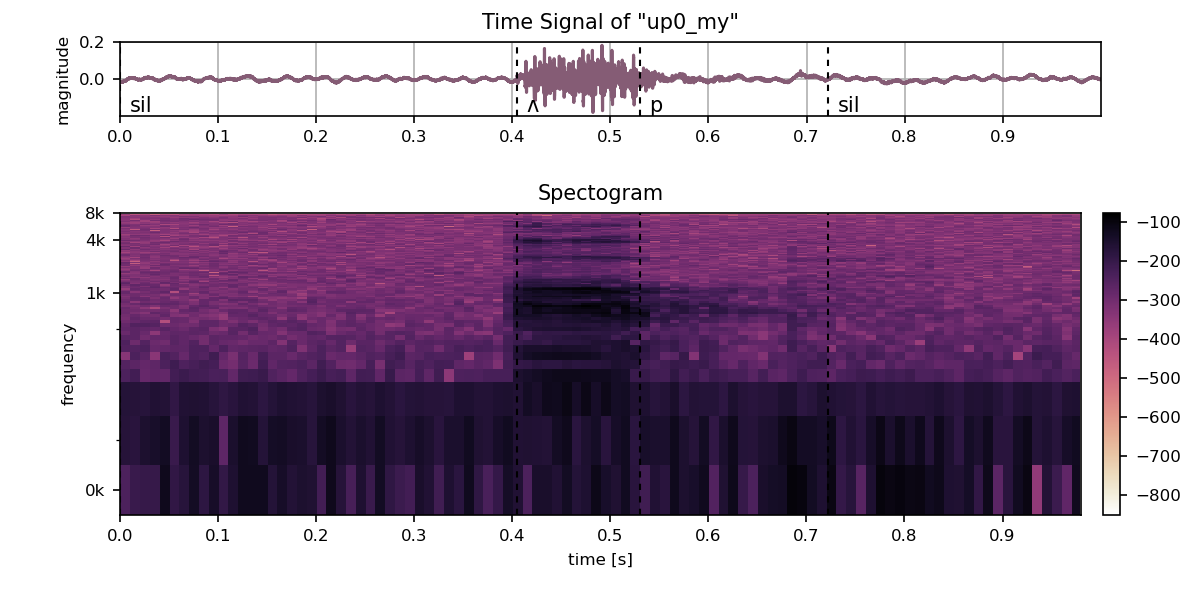
\includegraphics[width=0.45\textwidth]{./3_signal/figs/signal_spec-log_up0_my}}
    \subfigure[down]{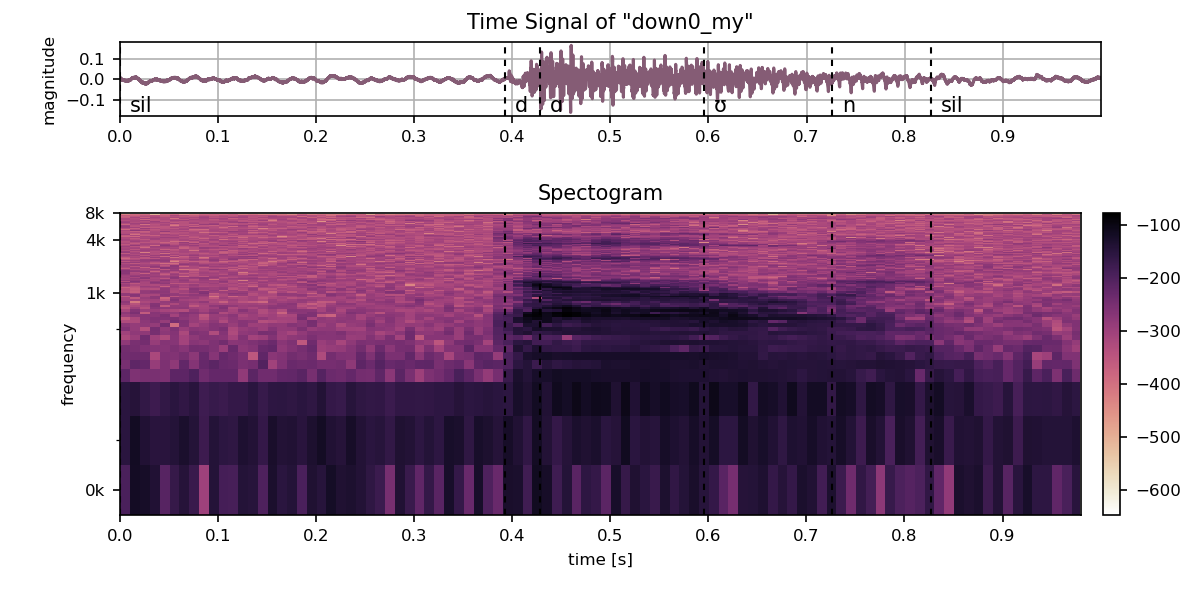
\includegraphics[width=0.45\textwidth]{./3_signal/figs/signal_spec-log_down0_my}}
    \subfigure[go]{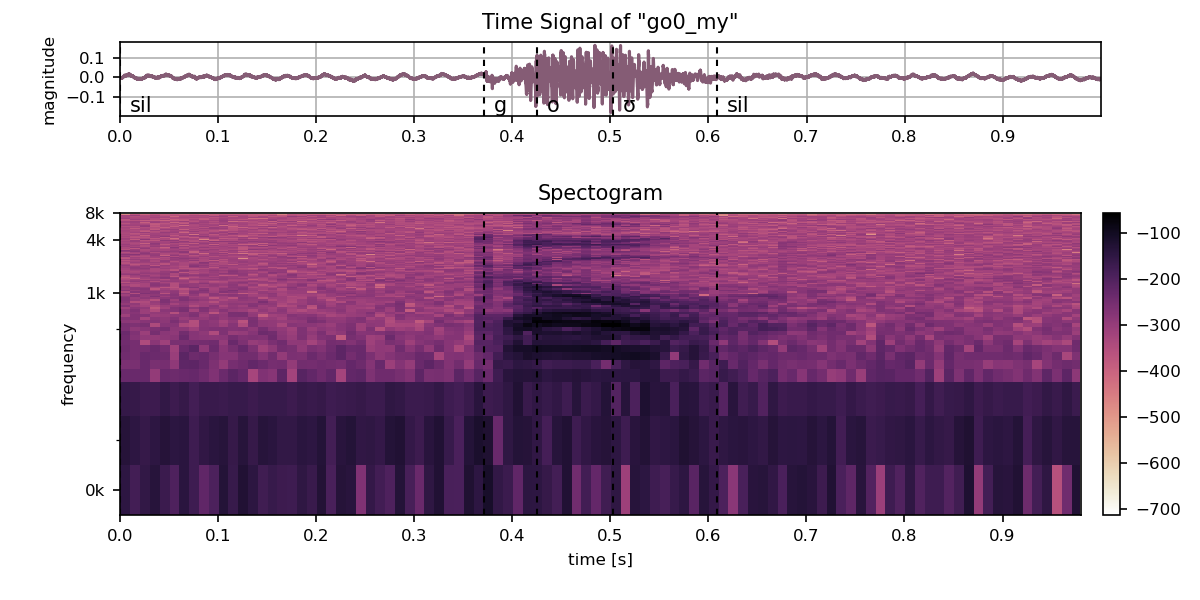
\includegraphics[width=0.45\textwidth]{./3_signal/figs/signal_spec-log_go0_my}}
  \caption{Spectogram logarithmic scaled.}
  \label{fig:spec-log}
\end{figure}
\FloatBarrier
\noindent